\section{Simulation numérique du modèle diffusif FHN}

\begin{frame}
\frametitle{Simulation numérique}
\framesubtitle{Équation de réaction‑diffusion de FitzHugh‑Nagumo}
\begin{itemize}
  \item Pour modéliser un tissu cardiaque, on étend le système à un domaine spatial : chaque point est un oscillateur FHN couplé aux voisins par diffusion.
  \item Le modèle devient une équation de réaction‑diffusion :
  \[
  \begin{cases}
    \displaystyle \frac{\partial v}{\partial t} = D \nabla^2 v + v - \frac{v^3}{3} - w + I_{\text{app}} \\[8pt]
    \displaystyle \frac{\partial w}{\partial t} = \varepsilon (v + a - b w)
  \end{cases}
  \]
  où $D$ est le coefficient de diffusion et $\nabla^2$ le laplacien spatial.
  \item Cette extension spatiale permet l’apparition d’ondes propagées et de structures auto‑entretenues comme les ondes spirales.
\end{itemize}
\end{frame}

\begin{frame}
\frametitle{Simulation numérique}
\framesubtitle{Discrétisation spatiale du laplacien}
\begin{itemize}
  \item Domaine carré $L\times L$ discrétisé par une grille régulière de $N\times N$ points, avec $\Delta x = L/(N-1)$.
  \item Conditions aux limites périodiques : les indices sont pris modulo $N$. Le bord gauche est voisin du bord droit, le bord supérieur du bord inférieur.
\end{itemize}
\end{frame}

\begin{frame}
\frametitle{Simulation numérique}
\framesubtitle{Conditions initiales pour l’onde spirale}
\begin{columns}
\column{0.45\textwidth}
\begin{itemize}
  \item Le tissu est initialement au repos ($v = v_{\text{repos}}$, $w = w_{\text{repos}}$).
  \item On excite un rectangle du domaine pour créer un front d’onde rectiligne.
  \item Ce front brisé s’enroule spontanément et forme une spirale stable après quelques rotations.
\end{itemize}
\column{0.55\textwidth}
\centering
\begin{figure}
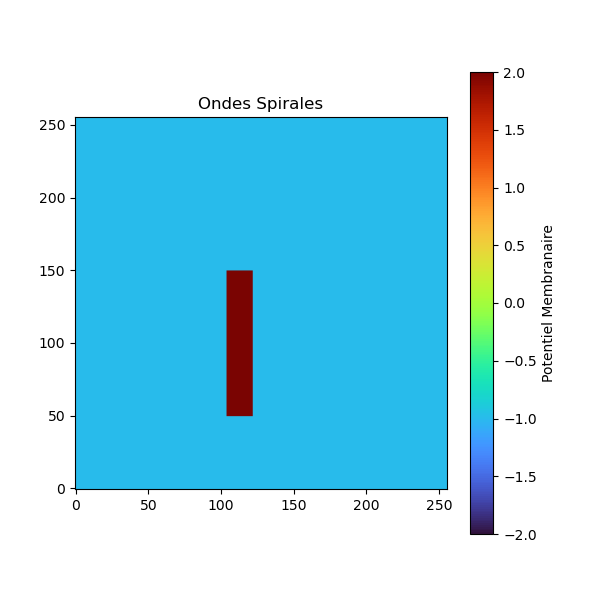
\includegraphics[width=\linewidth]{Figures/Potentiel.png}
\caption{État initial : domaine excité (rouge) et domaine au repos (bleu).}
\end{figure}
\end{columns}
\end{frame}

\begin{frame}
\frametitle{Simulation numérique}
\framesubtitle{Apparition d'une onde spirale}
\begin{columns}
\column{0.45\textwidth}
\begin{itemize}
  \item La pointe de la spirale tourne autour d’une zone centrale qui ne s’excite jamais.
  \item Le front d’onde parcourt le domaine périodiquement ; chaque point du tissu est excité une fois par rotation.
  \item Cette structure auto‑entretenue correspond aux réentrées fonctionnelles observées dans le myocarde.
\end{itemize}
\column{0.55\textwidth}
\centering
\begin{figure}
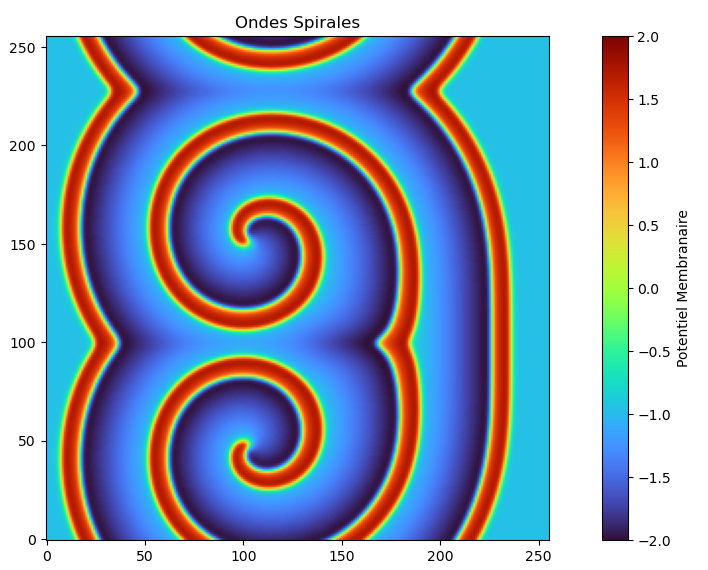
\includegraphics[width=\linewidth]{Figures/Spiral.png}
\caption{Instant de la simulation montrant l’onde spirale (échelle de couleurs : potentiel $v$).}
\end{figure}
\end{columns}
\end{frame}